\documentclass[format=sigconf]{acmart}
% \usepackage{usenix-2020-09}



\usepackage{enumitem}
\usepackage{subcaption}
% \usepackage{graphicx}
\usepackage{amsmath}
\usepackage{url}
\usepackage{color}
\usepackage{booktabs}
\usepackage{multirow}
\usepackage{algorithm}
\usepackage{algpseudocode}
\usepackage{tikz}
\usetikzlibrary{shapes.geometric,arrows,decorations.markings, arrows.meta}
\usetikzlibrary{positioning, calc}





% \raggedbottom
% 
\pagestyle{plain}
\begin{document}


\title{Attack Tree Edit Distance: refinement aware tree edit distance with semantic label replacement}

\iffalse{
    \author{Nathan D. Schiele}
    \orcid{0000-0003-1186-1503}
    \affiliation{\institution{Leiden University}
        \city{Leiden}
        \country{The Netherlands}}
    \email{n.d.schiele@liacs.leidenuniv.nl}


    \author{Olga Gadyatskaya}
    \orcid{0000-0002-3760-9165}
    \affiliation{\institution{Leiden University}
        \city{Leiden}
        \country{The Netherlands}}
    \email{o.gadyatskaya@liacs.leidenuniv.nl}
}\fi
\author{Anonymized for submission}




% \acmConference[FSE2024]{FSE2024}
% \acmYear{2024}
% %\acmBooktitle{Proceedings of the 32nd ACM Symposium on the Foundations of Software Engineering (FSE '24), November 15--19, 2024, Porto de Galinhas, Brazil}
% \acmBooktitle{Submission to FSE'24}

% \settopmatter{printfolios=true}

% \begin{teaserfigure}
%     \includegraphics[width=\textwidth]{img/Teaser02}
%     \caption{Participant created ADT}
%     \Description{A collage of ADTs that were created by participants}
%     \end{teaserfigure}

% \begin{teaserfigure}
% \includegraphics[width=\textwidth]{img/CollageTeaser}
% \caption{Assorted participant created ADTs}
% \Description{A collage of ADTs that were created by participants}
% \end{teaserfigure}


\begin{abstract}

    This is the abstract
\end{abstract}

\maketitle              % typeset the header of the contribution





\newcommand{\OG}[1]{{\color{blue} OG: #1}}
\newcommand{\NS}[1]{{\color{purple} NS: #1}}

\newcommand{\etal}{et al.}
\newcommand{\id}[2]{#1-#2}
\newcommand{\hypothesis}[1]{$\text{H}_\text{#1}$}
\newcommand{\RQ}[1]{\textbf{RQ#1}}

\newcommand{\ICS}{NCS}
\newcommand{\SEC}{CS}



\newcommand{\AND}{AND}
\newcommand{\SAND}{SAND}
\newcommand{\OR}    {OR}

\newcommand{\childFunc}[1]{\text{child}({#1})}
\newcommand{\parentFunc}[1]{\text{par}({#1})}

\newcommand{\ATnode}[2]{t_{{#1}.{#2}}}
\newcommand{\ATlabel}[2]{l_{{#1}.{#2}}}

\newcommand{\hResponse}[1]{\texttt{#1} - }

\newcommand{\anonfoot}{\footnote{Anonymized for submission}}


\newcommand{\qIndent}{4em}
\newcommand{\qsIndent}{2em}
\newcommand{\surveyq}[1]{\textbf{#1:}}





\section{Related Work}
\label{sec:related-work}

Distance between data structures is not a new concept. Many works have explored the idea of ``distance'' between strings. In string edit distance, where the difference in strings is given my a min-cost path taken by either adding a character, removing a character or replacing a character. By fining the minimum cost needed to transform one string into another, a ``distance'' value can be given. The cost of transformation increases with the difference between two strings~\cite{yujianNormalizedLevenshteinDistance2007, masekFasterAlgorithmComputing1980}.

Tree edit distance is seen as an extension of the string edit distance problem. Tai first tackled the problem, suggesting an edit distance metric for two directed acyclic graphs (DAG)s \cite{tai_tree--tree_1979}. Zhang and Shasha have written the seminal work on tree edit distance~\cite{zhang_simple_1989}. In their work, they describe a simple algorithm for calculating the distance between two trees. This algorithm is based on the idea of a \textit{forest} distance, which is the distance between two forests. A forest is possible disjoint a collection of trees, though a forest can consist of a single tree. The distance between two forests is the minimum cost of transforming one forest into another. This is calculated by finding the minimum cost of transforming each tree in the first forest into each tree in the second forest. This is done recursively until the minimum cost of transforming each node in the first tree into each node in the second tree is found. The minimum cost of transforming the first tree into the second tree is then given as the optimal \emph{tree edit distance} between two trees. This edit distance is given as both a value, the cost of the sequence of edits, as well as the sequence of edits itself. This sequence of edits has 3 possible operations.

Most of the research and development on tree edit distance focuses calculation optimization. As shown by Zhang~\etal, the tree edit distance problem for unordered trees is an \textit{NP}-Complete problem~\cite{zhang_editing_1992}. As such, the development of novel optimal calculation strategies is necessary to enable comparison of larger tree structures. Yoshino \etal\ developed a dynamic programming A$^*$ algorithm for computing unordered tree edit distance (UTED), which offer significant performance gains over exhaustive search~\cite{yoshino_dynamic_2013}. Their method uses an A$^*$ algorithm to construct a search tree of mappings. The distance is then calculated from these mappings. Unfortunately, these mapping rely on an absolute equivalence between nodes to establish a mapping, which will not exist in ``unfiltered'' attack trees, and thus cannot be applied in our case. However, the intuition to optimize finding mappings and then find the distance based on the mappings is a useful methodology that we can apply to our work. Other work based on the A$^*$ algorithm methodology, such as the optimizations offered by Paaßen~\cite{paasen_-algorithm_2021} for computing UTED will have the same unsuitability.

McVicar~\etal\ have developed a method of calculating UTED in SuMoTED by focusing on allowing nodes to move up or down a tree and organizing edits around a consensus tree~\cite{mcvicar_sumoted_2016}. This methodology allows them to achieved polynomial time calculation of UTED. However, application of this methodology to attack trees presents difficult. Namely, the same issue as the A$^*$ algorithm, the requirement of exact equivalence between node labels.

% McVicar~\etal\ have developed a method of calculating UTED in SuMoTED by focusing on allowing nodes to move up or down a tree and organizing edits around a consensus tree~\cite{mcvicar_sumoted_2016}. This methodology allows them to achieved polynomial time calculation of UTED. However, application of this methodology to attack trees presents difficult. Namely, the same disallowance of ordered nodes. Additionally, by allowing movement of nodes below leaf nodes would functionally introduce a refinement to the attack tree, which would require a new mechanism to accomodate this potential action. In effect, unlike SuMoTED, movement of nodes up a tree would not be equivalent to movement of nodes down a tree, and this equivalence is assumed in SuMoTED.

Pawlick and Augusten proposed RTED, a more optimal method of calculating ordered TED (OTED)~\cite{pawlik_rted_2011}. Their methodology is faster than Zhang and Shasha, but specifically for larger trees (500+ nodes). Attack trees by contrast cannot grow this large as they become unable as threat models~\cite{andersonSecurityEngineeringGuide2020}. As such, RTED, while an important optimization and contribution, does not offer a significant advantage for attack trees over Zhang and Shasha.

% Tree edit distance, like string edit distance, has a wide array of applications. Just as string edit distance has been used to compare sequences of DNA \NS{ cite},






% Much of the work in this field has built upon work by Kuo-Chung Tai who suggested that the distance between trees is similar to several previous works comparing the differences in strings~\cite{tai_tree--tree_nodate}.


% In the Zhang and Shasha algorithm the three possibilities for an edit operation between individual nodes are, (i) a node must be added, (ii) a node must be removed, or (iii) a node must be replaced~\cite{zhang_simple_1989}. Each of these operations has a cost

% Zhang and Shasha proposed a commonly cited simple algorithm for calculating tree edit distance~\cite{zhang_simple_1989}. We use this algorithm in this paper as it is a common strategy for implementing and testing extensions to tree edit distance. As such, optimizations based on the Zhang and Shasha algorithm can be applied to our methodology as we show in section \NS{When I write that section, I'll reference it here}.
\section{Requirements}
\label{sec:requirements}

The application of tree edit distance to attack trees requires a number of considerations. We outline these requirements in this section.


\subsection{Refinement Awareness}
\label{ssec:refinement}

The primary difference between attack trees and most directed acyclic graphs (DAGs) are the presence of refinements, or the given relationship between children. This is a critical part of the attack tree structure and must be included in the tree edit distance algorithm.

\subsection{Semantic Label Similarity}
\label{ssec:label-similarity}

In early iterations of tree edit distance problems, node labels were said to be equivalent if the labels were identical. However, in most contexts, it will not be the case that node labels will be identical. Especially in the context of cyber security, it is easily possible for two nodes in a DAG to represent the same idea but presented in a radically different manner. As such, the distance between attack trees must have a mechanism to account for the similarity between node labels on the basis of their meaning.

\subsection{Order of children}
\label{ssec:order-of-children}

It is a known problem that tree edit distance of unordered trees is an \textit{NP}-Complete problem~\cite{zhang_editing_1992}. However, attack trees are unique in that the order of children is dependent on the refinement of the parent node. As such, the distance between attack trees must be able to account for the order of children in the context of the refinement of the parent node. In the case of \AND\ and \OR\ refinements, the children are unordered. However, in the case of \SAND\ (\emph{Sequential} \AND) refinements, the order of children is important. As such, the edit distance between two attack trees must optimize to allow for the reordering of nodes when calculating the edit distance; however, this optimization must be such that it is selectively applicable, and can be not applied in the case of \SAND\ refinements.

\subsection{Metric}
\label{ssec:metric}

The distance between two attack trees must be a metric. That is to say, the distance between two attack trees must be non-negative, symmetric, and satisfy the triangle inequality.



\NS{I dunno if this should be included in this paper - but it'd make it SO MUCH EASIER to argue utility}
\subsection{Consensus Trees}
\label{ssec:consensus-trees}

One potential utility of tree edit distance would be to allow for the recognition missing vectors or components of attack trees \NS{cite AG distance paper}. For example, if we find that one tree is a whole subset of another tree, that is the consensus tree between two trees is equivalent to one of the trees, then we can infer that the components of the larger tree are components that would be directly applicable to the subset tree. As such, we can use this method of calculating a consensus tree to find missing components of attack trees.
\section{Refinement Awareness}

One of the biggest differences between attack trees and other tree-like data structures is the presence of refinements, or the \AND\ and \OR\ relationships, which state whether all of the children of a node must be satisfied for the parent node to be satisfiable (\AND) or if at least one must be satisfied for a parent node to be satisfiable (\OR).

The presence of refinements in a tree does not significantly complicate the calculation of tree edit distance. As given by RTED?, the tree edit distance can be given by the summation: \NS{include the nice summation from whatever paper I think I saw it in}.

In the Zhang and Shasha algorithm there are three possibilities for nodes, (i) a node must be added, (ii) a node must be removed, or (iii) a node must be replaced~\cite{zhang_simple_1989}, this is described as $\text { forestdist }\left(l\left(i_1\right) \ldots i, l\left(j_1\right) . . j\right)$. We give the cost of this change is given to be $\gamma(\Delta)$, then this cost would likewise need to be applied to all three cases. However, we find the following:

% Write a latex lemma environment in which the lemma shows that for the node removal case, there is no additional cost for changing a refinement, for the adding case, the cost of adding a refinment would be included in the cost of adding the node, and subsequently, the cost of replacing a node would have only the \gamma(\Delta)

\begin{lemma} \label{lem:refinement_change_cost} Let $T$ be an attack tree with $T = t\Delta(t_1,...,t_n)$ where $t = b|t\Delta(t_1,...,t_i)$ and $\Delta = \AND|\OR$. We give $b$ to be some action within the attack scenario. Let $\gamma$ be the cost function for the tree edit distance, with the cost of removing a subtree to be $\gamma(t_j \rightarrow {\Lambda})$, the cost of adding a subtree to be $\gamma({\Lambda}\rightarrow t_j)$, and the cost of changing a subtree to be $\gamma(t_j \rightarrow t_k)$. We give the cost changing a refinement for subtrees $t_i$ and $t_j$ to be $\gamma(\Delta_i \rightarrow \Delta_j)$ Then we have the following:

\begin{enumerate} 
      \item In the case of node removal, there can be no additional cost for changing a refinement. That is, if we remove a node $t_j$ from $T$, then we have:

            $$\gamma(t_j \rightarrow {\Lambda})$$

            $\Lambda$ is an empty tree, and by definition does not contain any refinements. Therefore, the cost of changing the refinement is zero.

      \item In the case of adding a node, the cost of adding a refinement would be included in the cost of adding the node. That is, if we add a node $t_j$ to $T$, then we have:

            $$\gamma(\Lambda \rightarrow {t_j})$$

            It is not possible to for a node in an attack tree to not have a refinement. If we allow

      \item In the case of replacing a node, the cost of replacing a refinement would be:

            $$\gamma({t_i} \rightarrow {t_j})$$

            This follows since the set of edges in $\mathcal{R}$ does not change when we replace $v$ with a new node $w$, but the number of edges in $G$ decreases by one

\end{enumerate}

    Therefore, we have shown that for any refinement $\mathcal{R}$ and any node removal, adding or replacing operation, the cost of changing the refinement is given by:

    $$\gamma(\mathcal{R}) = \gamma(V) - \gamma({(u, v) | u \in V \land v \in V})$$

    This holds for any graph $G$ and any function $\gamma$.

\end{lemma}

% \begin{multline*}
% \text { forestdist }\left(l\left(i_1\right) \ldots i, l\left(j_1\right) . . j\right)
% \\
% \text{  }\text{  }\text{  }=\min \left\{\begin{array}{l}
%         \text { forestdist }\left(l\left(i_1\right) \ldots i-1, l\left(j_1\right) . . j\right)+\gamma\left(T_1[i] \rightarrow \Lambda\right), \\
%         \text { forestdist }\left(l\left(i_1\right) . . i, l\left(j_1\right) . . j-1\right)+\gamma\left(\Lambda \rightarrow T_2[j]\right),    \\
%         \text { forestdist }\left(l\left(i_1\right) . . l(i)-1, l\left(j_1\right) . . l(j)-1\right)                                           \\
%         + \text { forestdist }(l(i) \ldots i-1, l(j) . . j-1)                                                                                 \\
%         +\gamma\left(T_1[i] \rightarrow T_2[j]\right) .
%     \end{array}\right.
% \end{multline*}




As the cost of replacing refinements is ever present, we can simply apply the cost of the replacing refinements after computing the tree edit distance by following the mappings and subsequently applying changed refinements. By doing this, we do not add to the time complexity of the Zhang and Shasha algorithm.

This method of computation works as it is not possible to have an intermediate attack tree node without a refinement~\cite{mauw_foundations_2006}. As such, all non-leaf nodes are either \AND\ or \OR\ nodes, so the distance between refinements is simple given as the cost needed to convert from one refinement to the other. As unlike the calculations of adding ($\Lambda \rightarrow i$), removing ($i \rightarrow \Lambda$), or replacement ($i \rightarrow j$), with refinements there is only on possible operation: replacement. Either \AND $\rightarrow$ \OR\ or \OR $\rightarrow$ \AND.

Similarly, \NS{the binary trees people}

Critically, this methodology can only work so long as the order of the nodes does not carry any significance (\textit{i.e} the nodes can be reordered without issue). There is an extention of attack trees which adds a sequential \AND\ (\SAND) refinement, in which the nodes in a \SAND\ relationship are given to be ordered~\cite{jhawar_attack_2015}; however, this is out of scope for our purposes. We discuss this further in Section~\NS{ref future work}.
\section{Semantic Label Replacement}

In tree edit distance, the replacement calculation is made when the root nodes of subtrees are not the same~\cite{zhang_simple_1989}. 


\tikzstyle{block} = [rectangle, draw, fill=black!290, 
    text width=5em, text=white,  text centered,  minimum height=4em]

    
\begin{figure*}
\begin{tikzpicture}[node distance = 2cm, auto]
    % Place nodes
    \node [xshift=-5cm](t1) {$T_1[i].\text{label}$};
    \node [below of = t1] (t2) {$T_2[j].\text{label}$};
    \node [block, below right = .5cm and 1cm of t1, yshift=.3cm]  (genbeddings) {\shortstack{Generate\\Semantic\\Embeddings}};
    \node [right of = t1, xshift=4cm]  (et1) {$\vec{e}(T_1[i].\text{label})$};
    \node [below of = et1]  (et2) {$\vec{e}(T_2[j].\text{label})$};
    \node [block, right of = genbeddings, xshift= 4.5cm]  (comp) {\shortstack{Vector\\Comparison}};
    \node [right of = comp, xshift = 2cm]  (end) {$\delta(T_1[i].\text{label}, T_2[j].\text{label})$};


    % Draw edges
    \draw [->] (t1.east)  -| ($(t1)!0.5!(genbeddings)$) coordinate |-(genbeddings);
    \draw [->] (t2.east)  -| ($(t2)!0.5!(genbeddings)$) coordinate |-(genbeddings);
    \draw [->] (genbeddings.east)  -| ($(genbeddings)!0.5!(et1)$) coordinate |-(et1);
    \draw [->] (genbeddings.east)  -| ($(genbeddings)!0.5!(et2)$) coordinate |-(et2);
    \draw [->] (et1.east)  -| ($(et1)!0.5!(comp)$) coordinate |-(comp);
    \draw [->] (et2.east)  -| ($(et2)!0.5!(comp)$) coordinate |-(comp);
    \draw [->] (comp)  -- (end);
\end{tikzpicture}
\caption{Process of calculating the distance between two node labels.}
\label{fig:semanticreplacement}
\end{figure*}




% One approach would be to ignore labels entirely and attempt to perform a tree edit comparison purely based on the structure of attack trees. This would be akin to setting the cost of replacement to 0. However, there is an additional issue as the Zhang and Shasha algorim relies on an initial mapping of like nodes between the two trees, a mapping done primarily based on labels. In order to ignore labels and define an edit distance based on tree structure alone, we would need to perform such a mapping based on the placement of nodes within the tree. Such a mapping would be possible

% , and would .  While this may yield interesting results, it can result in two trees being evaluated with an edit distance of 0 while not at all being similar (as they are structurally the same). A small example is provided in Figure~\NS{Add fig} where the two trees are structurally equivalent, and all that is needed to edit one tree to another would be to replace all nodes. If the cost of replacement is 0, then the edit distance between the two trees is likewise 0. 




\subsection{Semantic similarity}







% After performing this mapping step, we compute tree edit distance as described by Zhang and Shasha. However, the cost of replacing a node with another node is given as 1 - semantic similarity. In this way, nodes that have highly similar labels (a semantic similarity approaching 1) will have a low replacement cost, while those with little to no semantic similarity will have high replacement cost. Additionally, if we give that the cost of adding or removing a node to be 1, we prime the Zhang and Shasha algorithm to attempt to replace as many nodes as possible. \NS{this may not be a good thing}

\subsection{Semantic replacement}

The second use of semantic similarity is in the Zhang and Shasha replacement operation. In the provided algorithm, a label is comparison is made between the root nodes of two trees when calculating the cost of replacements. If the root node labels are the same, the cost of replacement is given as 0; otherwise the cost is given as 1. We adjust this label comparison by applying a semantic distance comparison.

We calculate the semantic embeddings for each node label, and compare the result embeddings. If the semantic similarity is above a given threshold, $\epsilon$, we give the cost of replacement to be 0; otherwise, we give the cost of replacement to be 1. This allows for the Zhang and Shasha algorithm to replace nodes with similar labels at a lower cost than nodes with dissimilar labels.

When we examine the forest distance equation from Zhang and Shasha~\cite{zhang_simple_1989}, we see the cost of replacing a given node as
% \begin{equation*}
\begin{align*}
    \text { forestdist } & \left(l\left(i_1\right) . . l(i)-1, l\left(j_1\right) . . l(j)-1\right) \\
                         & + \text { forestdist }(l(i) \ldots i-1, l(j) . . j-1)                   \\
                         & + \gamma\left(T_1[i] \rightarrow T_2[j]\right)
\end{align*}
% \end{equation*}


We give the $\gamma\left(T_1[i].\text{label} \rightarrow T_2[j].\text{label}\right)$ to be the following:

\begin{equation*}
    \gamma\left(T_1[i].\text{label} \rightarrow T_2[j].\text{label}\right)=\left\{\begin{array}{ll}
        0, & \text { if } \delta\left(T_1[i].\text{label}, T_2[j].\text{label}\right)>\epsilon \\
        1, & \text { otherwise }
    \end{array}\right.
\end{equation*}




% \begin{equation*}
%     \text { forestdist }\left(l\left(i_1\right) \ldots i, l\left(j_1\right) . . j\right)=\min \left\{\begin{array}{l}
%         \text { forestdist }\left(l\left(i_1\right) \ldots i-1, l\left(j_1\right) . . j\right)+\gamma\left(T_1[i] \rightarrow \Lambda\right), \\
%         \text { forestdist }\left(l\left(i_1\right) . . i, l\left(j_1\right) . . j-1\right)+\gamma\left(\Lambda \rightarrow T_2[j]\right),    \\
%         \text { forestdist }\left(l\left(i_1\right) . . l(i)-1, l\left(j_1\right) . . l(j)-1\right)                                           \\
%         + \text { forestdist }(l(i) \ldots i-1, l(j) . . j-1)                                                                                 \\
%         +\gamma\left(T_1[i] \rightarrow T_2[j]\right) .
%     \end{array}\right.
% \end{equation*}

Selecting the $\epsilon$ value will ultimately depend on the context in which this comparison is used.If $\epsilon$ is too lowe, then the cost of replacemenst will be 0 for all nodes, and the tree edit distance will be purely based on the structure of the treesa as all replacement operations will have no cost. If $\epsilon$ is too high, then the cost of replacement will be 1 for all nodes, and the tree edit distance will be identical to the original Zhang and Shasha algorithm (with all replacement operations having a cost of 1). In Figure~\ref{img:similaritylimits}, we show the average distance between the 38 experimental ATs per semantic similarity limit. We see that as the semantic similarity limit increases, the average distance between the trees increases, as the cost of all replacement operations slowly move toward 1. We discuss this further in Section~\ref{sec:results}
\section{Node Flipping}

The Zhang and Shasha edit distance algorithm is specifically given for ordered trees, that is, the order of child nodes is taken to be significant. In attack trees without sequential conjunction, the order of nodes is not given to be significant~\cite{mauw_foundations_2006,jhawar_attack_2015}. This results in an issue where trees with identical, but unordered nodes are given to have a high edit distance. This is shown in Figure~\ref{fig:nodeflipping}, where two trees with identical information but different node order are given to have a distance of 2. This is due to the fact that the Zhang and Shasha algorithm is not designed to handle unordered trees. Zhang and Jiang have shown that the tree edit distance problem for unordered trees is an MAX SNP-hard~\cite{zhangMAXSNPhardResults1994}. We suggest a novel method for handling tree edit distance in unordered attack trees by taking advantage of the inherent structure of attack trees.


\begin{figure}
    \begin{subfigure}{.45\linewidth}
        
\includegraphics[width=\linewidth]{img/NodeFlip1.png}
    \end{subfigure}
    \begin{subfigure}{.45\linewidth}
        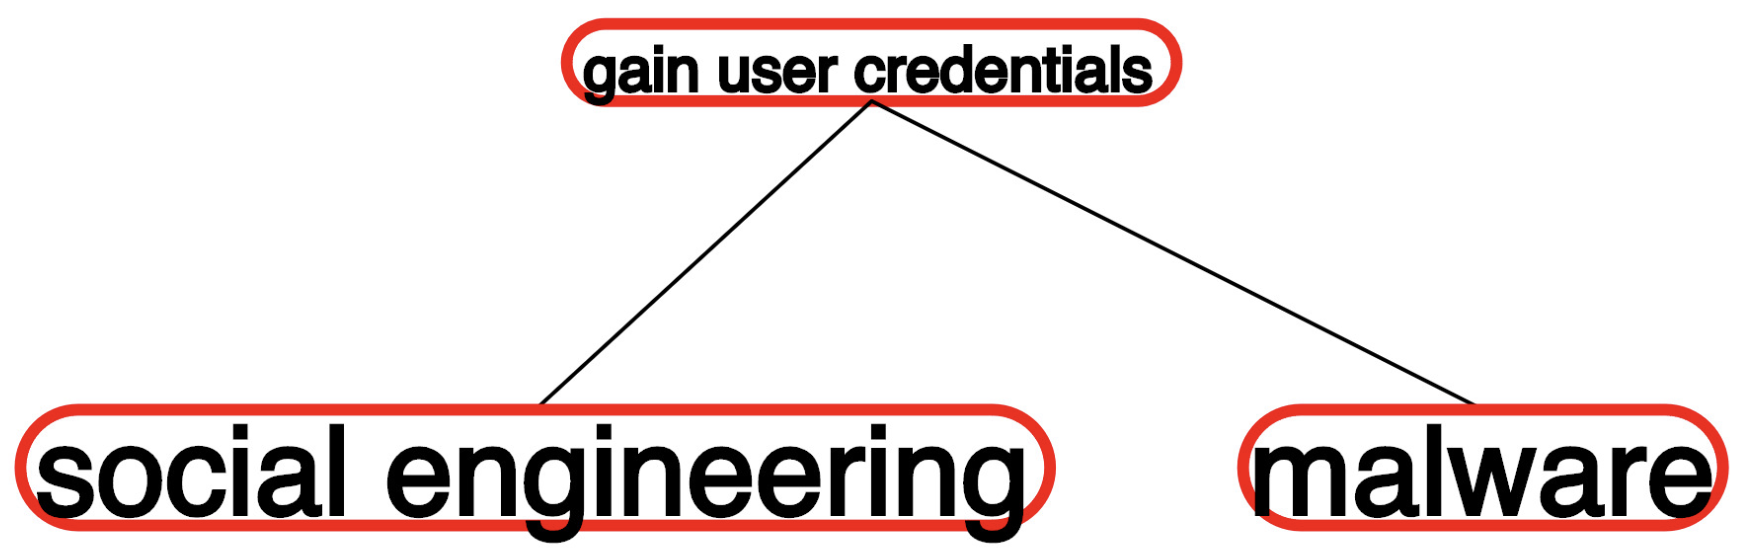
\includegraphics[width=\linewidth]{img/NodeFlip2.png}
    \end{subfigure}
    \caption{Two attack trees (subtrees of the example in Figure~\ref{fig:tartgetAT}) with identical information but different node order. These trees would evaluate to have a distance of 2 (two replacement operations).}
    \label{fig:nodeflipping}
\end{figure}

Attack trees, by virtue of their construction, tend to be organized in levels of abstraction. That is, with each new level of an attack tree, the nodes are given to be more specific than the nodes in the previous level. This is shown in Figure~\ref{fig:tartgetAT}, where the root node is given to be the most abstract (as the overall goal), while the leaf nodes are the most concrete (as the individual actions). From this, we find siblings in an attack tree to be on the same level of abstraction. As such, the order of siblings can be changed without affecting the meaning of the attack tree. By checking the order of sibling sets between the two attack trees




\subsection{Semantic mapping}

Zhang and Shasha motivate and validate their approach by creating a node mapping between the two trees (source and target)~\cite{zhang_simple_1989}. How this mapping is created was not a contribution of that work; however, simple rules for defining mappings based on node placement were included. For example, two nodes could only be mapped if they shared the same placement in terms of parents and siblings. A left-most sibling could not be mapped to a right-most sibling, even if they were the same node. This is part of the reasoning applied to establish that creating this mapping, and thus defining optimal tree-edit distance for unordered trees is an MAX SNP-hard problem~\cite{zhangMAXSNPhardResults1994}.

We adapt the idea of a mapping to instead map nodes based on a comparison of semantic label embeddings. Starting with the root nodes of both source and target trees, we create a matrix of all semantic similarities between the children of these nodes. Starting with the two nodes with the highest label semantic similarity, we map those two nodes together and remove the row and column corresponding to that value from the similarities matrix. Finally, we reorder the children in each tree such that mapped nodes have the same left-wise index. We then repeat this process until the similarities matrix is empty. We then repeat this process for all newly added mappings. This process is shown in Algorithm~\ref{alg:sibling_reorder}. It is a top down algorithm, starting from the root node and working down to the leaf nodes.

This methodology is not guaranteed to return smaller edit distance. If it were, this would represent a polynomial approximate solution to an MAX SNP-hard problem. We can construct a counter example by considering two trees with some identical subtree. If prior to the mapping the parent nodes of these subtrees were in the correct order such that these identical subtrees would be matched by the Zhang and Shasha algorithm, and the process of creating the semantic mapping caused the parent nodes of these identical subtrees to be placed out of order, the tree edit distance would increase as a result of our mapping step, as the previous matching operations (which are given to not have a cost) would no longer occur in the Zhang and Shasha algorithm, and would likely be replaced with a large series of add and remove operations (which each incur a cost). However, this scenario is only possible if the root nodes of these identical subtrees are not semantically mapped together, which is highly unlikely to occur in practice. This potential could be mitigated by calculating the tree edit distance twice: once with semantic node remapping and once without, to check that the node mapping has not increased edit distance. Such a step would not increase the computational complexity of the overall calculation, but would ensure that the worse case scenario does not occur.





\begin{algorithm}
    \caption{An algorithm to reorder siblings based on semantic similarity}
    \label{alg:sibling_reorder}
    \begin{algorithmic}
        \State Two attack trees $T_1$ and $T_2$ according to Definition~\ref{def:attack-tree} with $a$ and $b$ total nodes respectively
        \State $M$ is the mapping of nodes between $T_1$ and $T_2$ \Comment{We give $m[0]$ and $m[1]$ to be the source and target nodes of a mapping for $m \in M$}
        \State $M \gets T_1[a]\mapsto T_2[b]$\Comment{Root nodes are always mapped}
        \For{$m \in M$}

        \State $D \gets []$ \Comment{Matrix of semantic similarity values}
        \For{left-wise index $i$ in $m[0].\text{children}$}
            \For{leftwise index $j$ in $m[1].\text{children}$}
                \State $D[i][j] \gets$ 
                \State$\text{  }\text{  }\text{  }\text{  }\text{  }\text{  }\text{  }\text{  }\text{  }\delta(m[0].\text{children}[i].\text{label}, m[1].\text{children}[j].\text{label})$
            \EndFor
        \EndFor
        \State $M_t \gets \emptyset$ \Comment{Temporary set of mappings} 
        \While{$D$ is not empty}
            \State $i, j \gets \text{argmax}(D)$ \Comment{Largest value in $D$}
            \State $M_t \gets M_t \cup m[0].\text{children}[i]\mapsto m[1].\text{children}[j]$
            \State $D \gets D - i$ \Comment{Remove row $i$}
            \State $D \gets D - j$ \Comment{Remove column $j$}
        \EndWhile
        \For{$p$ in $M_t$}
            \If{indicies $i$, $j$ of $p$ are not equal}
                \State{Swap nodes $i$ and $j$ \textbf{in $T_1$}}
            \EndIf
        \EndFor
        \State $M \gets M \cup M_t$
        \EndFor
    \end{algorithmic}
    \end{algorithm}


    \subsection{Ordered Subtrees}

    As we have discussed in Sections~\ref{sec:background}~and~\ref{sec:refinement-awareness}, there are components of attack trees which can be given to be ordered; namely, \SAND\ attack trees~\cite{jhawar_attack_2015}. While these attack trees are out of scope for our definition and contribution, they are a common extension on the attack tree formalism~\cite{lallieReviewAttackGraph2020}. If a \SAND\ node exists within an attack tree, Algorithm~\ref{alg:sibling_reorder} can be modified to check the relationship between children of nodes and to directly map ordered nodes together regardless of label semantic similarity. As stated previously, this is out of scope for our contribution; the validation and testing of such an approach will have to be attended to in a future work.
\section{Methodology}
\label{sec:methodology}

We apply the validation methodology described in Section~\ref{sec:validation}.


\subsection{Theoretical Validation}
\label{ssec:methodology-examples}


Outside of the real-world experiment we developed to test the attack tree distance measurements, we also examine the distances measures with a series of theoretical examples. For these basic transformation examples (BTEs), we are not concerned with the semantic similarity,  as this is assessed in our experiment. As such, all labels are single capital letters and we set the similar limit ($\epsilon$) to 1, which would require node to be equivalent in order to be matched.

Each of these examples are simple enough that we can intuitively describe a distance. From this, we can examine how each of our distance measures handle each case. If a distance measure differs significantly from what we expect, this is indicative of the measure being deficient in measure some aspect of the distance between attack trees. The examples are shown in Figure~\ref{fig:counterexamples}.


\newcommand{\CEWidth}{.45\linewidth}
\begin{figure}
    \centering
\begin{subfigure}[b]{\linewidth}
        \centering
        \resizebox{2cm}{!}{
            \begin{forest}
    for tree={
    draw,
    minimum height=.25cm,
    anchor=parent,
    align=center,
    child anchor=parent,
    edge=-
    },
    adnode/.style={rounded rectangle,},
    [{R}, adnode,
            [{I}, adnode,  [{A}, adnode,] [{B}, adnode,]]
                [{J}, adnode, angle below, [{C}, adnode,] [{D}, adnode,]]
        ]
\end{forest}
        }
        \subcaption{Base Attack Tree}\label{sfig:base}
    \end{subfigure}
\begin{subfigure}[b]{\CEWidth}
        \centering
        \resizebox{2cm}{!}{
            \begin{forest}
        for tree={
        draw,
        minimum height=.25cm,
        anchor=parent,
        align=center,
        child anchor=parent,
        edge=-
        },
        adnode/.style={rounded rectangle,},
        [{R}, adnode,
                        [{J}, adnode, angle below, [{D}, adnode,] [{C}, adnode,]]
                                [{I}, adnode,  [{B}, adnode,] [{A}, adnode,]]
                ]
\end{forest}
        }
        \subcaption{Order Reversed}\label{fig:b}
    \end{subfigure}
\begin{subfigure}[b]{\CEWidth}
        \centering
        \resizebox{2cm}{!}{
            \begin{forest}
        for tree={
        draw,
        minimum height=.25cm,
        anchor=parent,
        align=center,
        child anchor=parent,
        edge=-
        },
        adnode/.style={rounded rectangle,},
        [{R}, adnode,
                        [{I}, adnode,  angle below, [{A}, adnode,] [{B}, adnode,]]
                                [{J}, adnode,  [{C}, adnode,] [{D}, adnode,]]
                ]
\end{forest}
        }
        \subcaption{Refinements Switched}\label{fig:b}
    \end{subfigure}
\begin{subfigure}[b]{\CEWidth}
        \centering
        \resizebox{2cm}{!}{
            \begin{forest}
        for tree={
        draw,
        minimum height=.25cm,
        anchor=parent,
        align=center,
        child anchor=parent,
        edge=-
        },
        adnode/.style={rounded rectangle,},
        [{R}, adnode,
                        [{I}, adnode, [{I}, adnode,  [{A}, adnode,] [{B}, adnode,]]]
                                [{K}, adnode]
                                [{J}, adnode, angle below, [{C}, adnode,] [{D}, adnode,]]
                ]
\end{forest}
        }
        \subcaption{Extra Intermediate}\label{fig:b}
    \end{subfigure}
\begin{subfigure}[b]{\CEWidth}
        \centering
        \resizebox{2cm}{!}{
            \begin{forest}
        for tree={
        draw,
        minimum height=.25cm,
        anchor=parent,
        align=center,
        child anchor=parent,
        edge=-
        },
        adnode/.style={rounded rectangle,},
        [{R}, adnode, [{A}, adnode,] [{B}, adnode,]
                                [{J}, adnode, angle below, [{C}, adnode,] [{D}, adnode,]]
                ]
\end{forest}
        }
        \subcaption{Missing Intermediate}\label{fig:b}
    \end{subfigure}
\begin{subfigure}[b]{\CEWidth}
        \centering
        \resizebox{2.5cm}{!}{
            \begin{forest}
        for tree={
        draw,
        minimum height=.25cm,
        anchor=parent,
        align=center,
        child anchor=parent,
        edge=-
        },
        adnode/.style={rounded rectangle,},
        [{R}, adnode,
                        [{I}, adnode,  [{A}, adnode,] [{B}, adnode,][{E}, adnode,]]
                                [{J}, adnode, angle below, [{C}, adnode,] [{D}, adnode,]]
                ]
\end{forest}
        }
        \subcaption{Extra Leaf}\label{fig:b}
    \end{subfigure}
\begin{subfigure}[b]{\CEWidth}
        \centering
        \resizebox{2cm}{!}{
            \begin{forest}
        for tree={
        draw,
        minimum height=.25cm,
        anchor=parent,
        align=center,
        child anchor=parent,
        edge=-
        },
        adnode/.style={rounded rectangle,},
        [{R}, adnode,
                        [{I}, adnode,  [{A}, adnode,] ]
                                [{J}, adnode, angle below, [{C}, adnode,] [{D}, adnode,]]
                ]
\end{forest}
        }
        \subcaption{MissingLeaf}\label{fig:b}
    \end{subfigure}
\begin{subfigure}[b]{\CEWidth}
        \centering
        \resizebox{2cm}{!}{
            \begin{forest}
        for tree={
        draw,
        minimum height=.25cm,
        anchor=parent,
        align=center,
        child anchor=parent,
        edge=-
        },
        adnode/.style={rounded rectangle,},
        [{Z}, adnode,
                        [{I}, adnode,  [{A}, adnode,] [{B}, adnode,]]
                                [{J}, adnode, angle below, [{C}, adnode,] [{D}, adnode,]]
                ]
\end{forest}
        }
        \subcaption{Changed Root}\label{fig:b}
    \end{subfigure}
\begin{subfigure}[b]{\CEWidth}
        \centering
        \resizebox{2cm}{!}{
            \begin{forest}
        for tree={
        draw,
        minimum height=.25cm,
        anchor=parent,
        align=center,
        child anchor=parent,
        edge=-
        },
        adnode/.style={rounded rectangle,},
        [{R}, adnode,
                        [{K}, adnode,  [{A}, adnode,] [{B}, adnode,]]
                                [{J}, adnode, angle below, [{C}, adnode,] [{D}, adnode,]]
                ]
\end{forest}
        }
        \subcaption{Changed Intermediate}\label{fig:b}
    \end{subfigure}
\begin{subfigure}[b]{\CEWidth}
        \centering
        \resizebox{2cm}{!}{
            \begin{forest}
        for tree={
        draw,
        minimum height=.25cm,
        anchor=parent,
        align=center,
        child anchor=parent,
        edge=-
        },
        adnode/.style={rounded rectangle,},
        [{R}, adnode,
                        [{I}, adnode,  [{E}, adnode,] [{B}, adnode,]]
                                [{J}, adnode, angle below, [{C}, adnode,] [{D}, adnode,]]
                ]
\end{forest}
        }
        \subcaption{Changed Leaf}\label{fig:b}
    \end{subfigure}
\begin{subfigure}[b]{\CEWidth}
        \centering
        \resizebox{2cm}{!}{
            \begin{forest}
        for tree={
        draw,
        minimum height=.25cm,
        anchor=parent,
        align=center,
        child anchor=parent,
        edge=-
        },
        adnode/.style={rounded rectangle,},
        [{R}, adnode,
                        [{I}, adnode,  [{A}, adnode,] ]
                                [{J}, adnode, angle below, [{B}, adnode,][{C}, adnode,] [{D}, adnode,]]
                ]
\end{forest}
        }
        \subcaption{Move Adjacent}\label{fig:b}
    \end{subfigure}
\begin{subfigure}[b]{\CEWidth}
        \centering
        \resizebox{2cm}{!}{
            \begin{forest}
        for tree={
        draw,
        minimum height=.25cm,
        anchor=parent,
        align=center,
        child anchor=parent,
        edge=-
        },
        adnode/.style={rounded rectangle,},
        [{R}, adnode,
                        [{I}, adnode,  [{A}, adnode,] ]
                                [{B}, adnode,]
                                [{J}, adnode, angle below, [{C}, adnode,] [{D}, adnode,]]
                ]
\end{forest}
        }
        \subcaption{Move Up}\label{fig:b}
    \end{subfigure}
\begin{subfigure}[b]{\CEWidth}
        \centering
        \resizebox{1.8cm}{!}{
            \begin{forest}
        for tree={
        draw,
        minimum height=.25cm,
        anchor=parent,
        align=center,
        child anchor=parent,
        edge=-
        },
        adnode/.style={rounded rectangle,},
        [{R}, adnode,
                        [{I}, adnode,  [{A}, adnode,[{B}, adnode,]] ]
                                [{J}, adnode, angle below, [{C}, adnode,] [{D}, adnode,]]
                ]
\end{forest}
        }
        \subcaption{Move Down}\label{fig:b}
    \end{subfigure}
\caption{Basic Transformation Examples (BTEs)}\label{fig:counterexamples}
\end{figure}





\subsection{Experimental Validation}

\subsubsection{Experimental Study Design}
\label{ssec:method-study-design}

Students were assigned a project related to attack defense trees as a part of their regular coursework. The project was a mandatory, graded assignment. Students had the option to provide consent for their anonymized responses to be collected for research purposes, this is described in detail in Section~\ref{ssec:ethics}. The assignment consisted of four components. In each component, students were required to create an attack (defense) tree (ADT) using a web application of our own design. Of the four components, the third was included in the assignment for the purposes of validating our approach. The text of the entire study is included in Appendix~\ref{app:exp-questions}; however, we only expound upon the relevant section in this work.

The third component of the study contains two parts. In part A, students were tasked with creating an AT from a provided, written, scenario. The scenario was adapted from an attack tree shown in Naik~\etal~\cite{naikEvaluationPotentialAttack2022}. The scenario was as follows:

\texttt{Many attackers aim to obtain personal data. Gathering personal data can be completed through unauthorized access to profile, credential creep, or a background data attack. Unauthorized access to profile requires gaining user credentials and accessing the profile. The credentials can be gained through a malware attack or a social engineering attack, and the profile can be accessed by stealing a phone or by remote access. Credential creep can be completed by submitting a request for additional data other than what is needed for verification or by user profiling. Finally, a background data attack requires both obtaining a sensitive dataset and linking the dataset via a request for verification.}

This description was created by reading the attack tree in Naik~\etal\ abstraction level by abstraction level, always going from left to right~\cite{naikEvaluationPotentialAttack2022}. The intention of Part A was to assess the requirements of unfiltered labels as well as processing the structure of the attack tree, as the underlying information in the attack trees should be identical between students. As the trees were effectively the same tree, distance between them would more likely be due to an artifact of the distance measure as opposed to the actual distance present in the data. By examining this, we would be able to validate our approach.

We then asked students in part B to expand upon their attack tree by ``doing your own research, add at least 5 new nodes and 2 new refinements to the attack tree you created in the previous section''. In all, this creates a relatively predictable, yet varied, dataset. In Part A, all trees should roughly be the same, baring minor changes in the label of nodes or the order of nodes. We expect that any large differences in part A to be due to misunderstanding the assignment or misreading the scenario. As Part B is built from each students' part A, we expect that the ``core'' of their attack tree to remain unchanged but the added nodes and refinement should introduce an ability to evaluate edit distance. Based on previous experience with similar studies, we expect most students to add exactly 5 new nodes and 2 new refinements, which should allows for some predictable edit distance (namely, the cost of adding 5 new nodes). This allows us to evaluate the distance measures as a metric, as well as further validation. As each student produced two trees, a base and an extension, by comparing them we can validate the distance measures. As if the distance measures are not able to recognize the base tree, the distance measure may not be suitable.

\subsubsection{Analysis}
\label{ssec:method-analysis}
From the first task (AT1), we would expect all trees to be roughly equal. There may be some variation due to missing or added information, from participants who may have deviated from the instructions. We would expect for the average distance of all AT1 trees to remain the same for increasing values of $\epsilon$. From this, we can establish ideal values of $\epsilon$, as once the average distance starts increasing, values that were previously equivalent and likely should be equivalent will start to rise. We can further validate by comparing AT1 to AT2 per participant, as these graphs should be constant for any value of $\epsilon$, as the only difference should be added nodes and added nodes are unaffected by the semantic similarity limit (as added nodes will always have a distance of 1). If the distance measures comparing AT1 to AT2 are not constant for all values of $\epsilon$, this would indicate a distance measure that behaves in an unexpected and potentially invalid manner. Finally, by comparing the difference distance measures on AT2, which are truly different attack trees, we can see if the distance measures behave similarly. Ideally, distance measures incorporate all aspects of attack trees, so their behavior should be similar. If the distance measures do not behave similarly, it may be a sign of an invalid distance measure. Our code for all distance algorithms and analysis is provided here: \url{https://anonymous.4open.science/r/ATD-FB1F/README.md}.

\paragraph{Web Application}

For this assignment, we created a web application which can be used to create attack defense trees. The web application contains a graphic interface with which users can add, delete and modify nodes~\cite{mohalaiaImplementingUserInterface2023}. Additionally, the web application contains an SQL-like language that can be used to generate ADTs~\cite{mezaADTLangDeclarativeLanguage2023}. The Web application additionally allows users to download ADTs as images as well as in the ADTool XML schema as defined by Kordy~\etal~\cite{kordy_adtool_2013}. The web application can be found here: \url{https://anonymous.4open.science/w/ADT-Web-App-AB3C/}.

\subsubsection{Participants}
The participants in this study were all third year bachelor students taking part in a minor on cyber security and governance. Most students were in policy related majors such as Security Studies or International Relations. The participants on average had only a few months of programming experience, which was a result of another course in the minor. Students were asked if they had any prior knowledge of threat models or attack trees, and only a few students had any prior knowledge. Students took this course in the fall semester of 2023. As shown by Naiakshina~\etal\ and Karpati~\etal, in the context of cyber security, students are a sufficient proxy for practitioners~\cite{karpatiComparingAttackTrees2014, naiakshinaConductingSecurityDeveloper2020}.



% \subsubsection{Processing}

% The attack tree data was collected in the form of XML data. This data was then processed using a Python script. The script was used to extract the attack trees from the XML data and to convert the attack trees into a format that could be used by our implementation of the Zhang and Shasha algorithm. We started with the pre-implemented and tested \texttt{zss} library from Tim Henderson~\cite{hendersonZssTreeEdit}. We then modified the library to include our semantic label replacement cost and refinement change cost to create an implementation of the Zhang and Shasha algorithm that should be effective for attack trees. We subsequently used this implementation to calculate the tree edit distance between the attacks trees.  

% Our code for all distance algorithms is provided here: \url{https://anonymous.4open.science/r/ATD-FB1F/README.md}.


\subsubsection{Sentence Embeddings}
\label{ssec:method-embeddings}

As we discussed in Section~\ref{sssec:semantic-similarity}, BERT is a state-of-the-art method for creating sentence embeddings. We use the \texttt{SentenceTransformers} library to calculate the sentence embeddings and cosine similarity to calculate embedding vector difference. As stated previously, our contribution is not the creation of these embeddings; additionally, our use of sentence embeddings is method agnostic, and any method for generating sentence or word embeddings could be used with our methodology. We used multiple different pre-trained BERT models and aggregated the results to illustrate that any results we found were not the result of the use of a specific model. Additionally, we did not fine tune any model. We used the following models: \texttt{paraphrase-multilingual-MiniLM-L12}, \texttt{all-mpnet-base}, and \texttt{all-MiniLM-L12}.

\subsubsection{Ethics}
\label{ssec:ethics}
This study was approved by the the Ethics Review Board at a european university\anonfoot. Students were informed of study and were requested to give consent for their responses to be included in the study. Multiple safeguards were used to ensure that students did not feel pressured into giving consent, as the assignment was a mandatory course component. Students were informed that they could withdraw their consent at any time, and that their responses would be anonymized. 







\section{Results}

\begin{figure}
    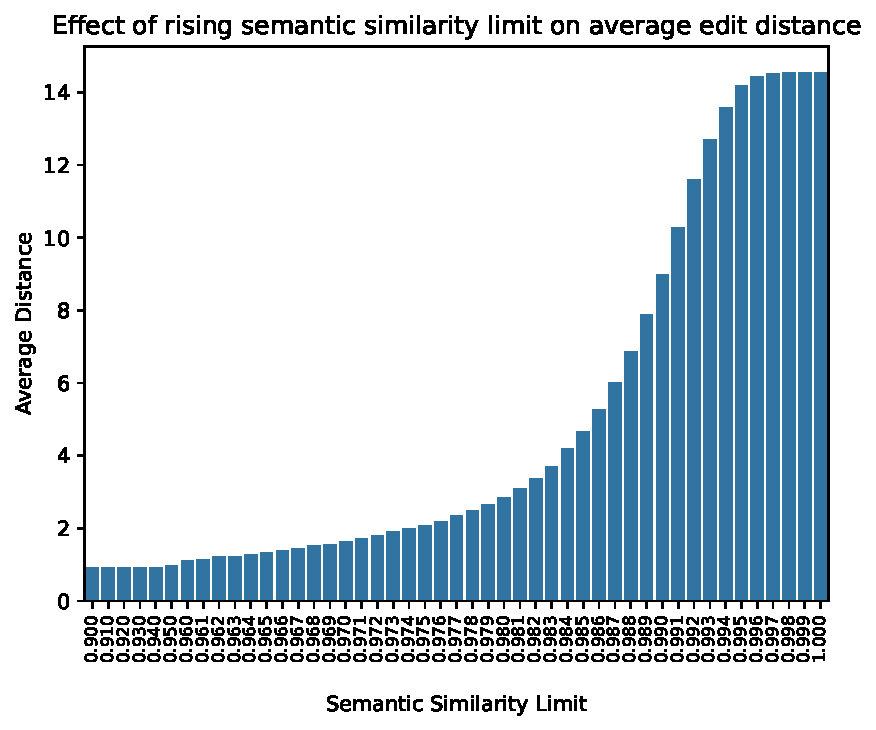
\includegraphics[width=\linewidth]{code/img/similaritylimits.pdf}
\end{figure}



\cite{*}



\bibliography{bibliography}{}
\bibliographystyle{plain}



\appendix
% \section*{Appendix}



\section{Proofs}
\label{appendix:proofs}
\subsection{Proof of Lemma~\ref{lem:gamma-delta}}
\label{appendix:lem:gamma-delta}
\begin{proof}


    \begin{enumerate}
        \item In the case of node removal, there can be no additional cost for changing a refinement. That is, if we remove a node $\ATnode{d}{i}$ from $T$, then we have:

              $$\gamma(\ATnode{d}{i} \rightarrow {\Lambda})$$

              $\Lambda$ is an empty tree, and by definition does not contain any refinements. Therefore, the cost of changing the refinement is zero.

        \item In the case of adding a node, the cost of adding a refinement would be included in the cost of adding the node. That is, if we add a node $\ATnode{d}{i}$ to $T$, then we have:

              $$\gamma(\Lambda \rightarrow {\ATnode{d}{i}})$$

              It is not possible to for a node in an attack tree to not have a refinement. If we separate the cost of adding a node and the cost of adding a refinement, we have one of the two following cases:
              \begin{enumerate}
                  \item A node is added without a refinement, which gives a refinement addition cost of 0, but results in an attack tree which is not valid given our attack tree definition.
                  \item The cost of adding a refinement is \textbf{always} added to the cost of adding a node, which results in the new cost of adding a node to always include $\gamma(\Delta)$.
              \end{enumerate}

              Given one of these cases results in an invalid tree, the other case must always apply. Therefore, by convention, we do not separate the cost of adding a node and the cost of adding a refinement, these are one and the same.

        \item In the case of replacing a node, the cost of replacing a refinement would be:

              $$\gamma({\ATnode{d}{i}} \rightarrow {\ATnode{e}{j}})$$

              Which we declare to consist of the sum following two costs:

              $$\gamma({\ATlabel{d}{i}} \rightarrow {\ATlabel{e}{j}})$$

              Which is the cost of changing one label to another. This is the original cost of replacing a node according to Zhang-Shasha. We also have:

              $$\gamma(\Delta)$$

              Which as previously stated is the cost of changing a refinement.



    \end{enumerate}

\end{proof}

\subsection{Proof of Lemma~\ref{lem:gamma-delta-2}}
\label{appendix:lem:gamma-delta-2}

\begin{proof}
    Let $T$ be an attack tree.

    Assume that $\gamma(\Delta) > \gamma(\ATnode{e}{j} \rightarrow {\Lambda}) + \gamma(\Lambda \rightarrow {\ATnode{e}{j}})$.

    Let $S$ be the optimal sequence of edit operations according to the Zhang-Shasha algorithm. That is, $\gamma(S)$ is minimal for all possible edit sequences for $\delta(T_1, T_2)$ Let some operation $s \in S$ be an operation to replace some node, $\ATnode{d}{i}$, with another, $\ATnode{e}{j}$.

    Thus, $\gamma(s) = \gamma({\ATlabel{d}{i}} \rightarrow {\ATlabel{e}{j}}) + \gamma(\Delta)$

    We have two cases:

    \begin{enumerate}
        \item $\ATnode{d}{i}.\Delta = \ATnode{e}{j}.\Delta$

              In this case, both $\ATnode{d}{i}$ and $\ATnode{e}{j}$ have the same refinement. Thus, $\gamma(\Delta) = 0$. Therefore, $\gamma(s) = \gamma({\ATlabel{d}{i}} \rightarrow {\ATlabel{e}{j}})$.

        \item $\ATnode{d}{i}.\Delta \ne \ATnode{e}{j}.\Delta$

              In this case, both $\ATnode{d}{i}$ and $\ATnode{e}{j}$ have different refinements. Thus, $\gamma(\Delta) > 0$. Therefore, $\gamma(s) = \gamma({\ATlabel{d}{i}} \rightarrow {\ATlabel{e}{j}}) + \gamma(\Delta)$.

              However, we have assumed that $\gamma(\Delta) > \gamma(\ATnode{e}{j} \rightarrow {\Lambda}) + \gamma(\Lambda \rightarrow {\ATnode{e}{j}})$. Therefore, $\gamma(s) = \gamma({\ATlabel{d}{i}} \rightarrow {\ATlabel{e}{j}}) + \gamma(\Delta) > \gamma(\ATnode{e}{j} \rightarrow {\Lambda}) + \gamma(\Lambda \rightarrow {\ATnode{e}{j}})$, as by convention $\gamma$ cannot result in a negative value.

              As such, we can replace $s$ with the sequence of operations $s_1$ and $s_2$, where $s_1$ is the operation to remove $\ATnode{d}{i}$ and $s_2$ is the operation to add $\ATnode{e}{j}$. Thus, $\gamma(s_1) = \gamma(\ATnode{e}{j} \rightarrow {\Lambda})$ and $\gamma(s_2) = \gamma(\Lambda \rightarrow {\ATnode{e}{j}})$. Therefore, $\gamma(s_1) + \gamma(s_2) < \gamma(s)$.

              This results in a contradiction, as $S$ is the optimal sequence of edit operations according to the Zhang-Shasha algorithm, it must not be possible to replace any $s \in S$ with an operation, or sequence of operations, with lower cost.
    \end{enumerate}

    Therefore, if $\gamma(\Delta) > \gamma(\ATnode{e}{j} \rightarrow {\Lambda}) + \gamma(\Lambda \rightarrow {\ATnode{e}{j}})$, then $\gamma(\Delta)$ either must be 0 for a change node edit operation to be included in the optimal sequence of edit operations (case 1), or the optimal sequence of edit operations must always result in node removal then replacement (case 2). In both cases, $\gamma(\Delta)$ is not used.

    Therefore, in order to include the cost of changing refinements in the cost of replacing a node, it must be the case that $\gamma(\Delta) \le \gamma(\ATnode{e}{j} \rightarrow {\Lambda}) + \gamma(\Lambda \rightarrow {\ATnode{e}{j}})$.


\end{proof}



























\section{Experiment Questions}
\label{app:exp-questions}


% \subsection*{ADT 1: Assembling ADTs}

% The following attack \textbf{leaf} nodes are provided. The overall goal of this scenario (and thus the root node of the tree) is \textbf{Rob bank}. Assemble an attack-defense tree using these leaf nodes. Do not add any additional leaf nodes. You may add any intermediary nodes you wish.

% \textbf{Attack leaf nodes:}
% % Why the fuck is there so much space here?
% % \vspace{-10cm}
% % \begin{itemize}
% %   \item Hire Outright
% %   \item Promise part of the stolen money
% %   \item Threaten insiders

% %   \item Buy tools
% %   \item Steal tools
% %   \item Gain Access
% %   \item Walk through front door
% %   \item Locate start of tunnel
% %   \item Find direction to tunnel
% % \end{itemize}

% Hire Outright, Promise part of the stolen money, Threaten insiders, Buy tools, Steal tools, Gain Access, Walk through front door, Locate start of tunnel, Find direction to tunnel

% \textbf{Defense leaf nodes:}

% Personnel Risk Management, Check employee financial situation


% \subsection*{Perception Questions}


% \subsubsection*{Likert Questions}
% \begin{itemize}
%   \setlength{\itemindent}{\qIndent}
%   \item[\surveyq{LS-ADT1-L1}] I find the structure of attack tree easy to understand
%   \item[\surveyq{LS-ADT1-L2}] Given all the nodes of an attack tree, it is easy for me to assemble the tree
%   \item[\surveyq{LS-ADT1-L3}] Given only the leaf nodes of an attack tree, it is easy for me to assemble the tree.
%   \item[\surveyq{LS-ADT1-L4}] I would rather define my own intermediary nodes
%   \item[\surveyq{LS-ADT1-L5}] The process of assembling the attack tree helped me better understand the attack scenario.
% \end{itemize}

% \subsubsection*{Short Response Questions}
% \begin{itemize}
%   \setlength{\itemindent}{\qIndent}
%   \item[\surveyq{LS-ADT1-W1}] What did you find most difficult about this task? Why?
%   \item[\surveyq{LS-ADT1-W2}] How did you go about solving this task? What was your methodology?
% \end{itemize}



% \subsection*{ADT 2: Building ADTs}

% The following text scenario is provided for you. Please create a complete attack defense tree \textbf{of this scenario}. \textbf{Do not add extra information that is not in the scenario}. Try to encapsulate the entire scenario with an attack-defense tree (don't leave any aspect of the attack scenario out).

% \emph{Scenario:} 
% The goal is to open a safe. To open the safe, an attacker can pick the lock,
% learn the combination, cut open the safe, or install the safe improperly so
% that he can easily open it later. Some models of safes are such that they cannot be picked, so if this model is used, then an attacker is unable to pick the lock. There are also auditing services to check if safes and other security technology is installed correctly. To learn the combination, the attacker
% either has to find the combination written down or get the combination
% from the safe owner. If the password is such that the safe owner can remember it, then the safe owner would not need to write it down.



% \subsection*{Perception Questions}

% \subsubsection*{Likert Questions}
% \begin{itemize}
%   \setlength{\itemindent}{\qIndent}
%   \item[\surveyq{LS-ADT2-L1}] I prefer reading attack trees to text descriptions of attacks.
%   \item[\surveyq{LS-ADT2-L2}] The process of building the attack tree helped me better understand the attack scenario.
% \end{itemize}

% \subsubsection*{Short Response Questions}
% \begin{itemize}
%   \setlength{\itemindent}{\qIndent}
%   \item[\surveyq{LS-ADT2-W1}] What did you find most difficult about this task? Why?
%   \item[\surveyq{LS-ADT2-W2}] How did you go about building the ADT?\@ What was your methodology?
%   \item[\surveyq{LS-ADT2-W3}] What was the first node you added to your tree?
% \end{itemize}


% \subsection*{ADT 3: Using Attack Trees}
This question is slightly different than the other questions. You need to create attack trees only. \textbf{This means you should NOT use defense nodes at all for this question}. In Part I, raw an attack tree from the provided scenario; \textbf{include all information from the scenario, do not include information that is not in the scenario}. In Part II, add onto the provided attack tree with new nodes and refinements that you find through your own research.

\subsection*{AT1: Attack tree from scenario}

\emph{Scenario:}  Many attackers aim to obtain personal data. Gathering personal data can be completed through unauthorized access to profile, credential creep, or a background data attack. Unauthorized access to profile requires gaining user credentials and accessing the profile. The credentials can be gained through a malware attack or a social engineering attack, and the profile can be accessed by stealing a phone or by remote access. Credential creep can be completed by submitting a request for additional data other than what is needed for verification or by user profiling. Finally, a background data attack requires both obtaining a sensitive dataset and linking the dataset via a request for verification. 


\subsection*{AT2: Finding new attack components}

Doing your own research, add at least 5 new nodes and 2 new refinements to the attack tree you created in the previous section.





\subsection*{Perception Questions}

\subsubsection*{Likert Questions}
\begin{enumerate}
    \setlength{\itemindent}{\qIndent}
  \item[\surveyq{LS-ADT3-L1}] I prefer reading attack trees to text descriptions of attacks.
  \item[\surveyq{LS-ADT3-L2}] The process of building the attack tree helped me better understand the attack scenario.
  \item[\surveyq{LS-ADT3-L3}]  The ADT communicates the attack scenario better than the written scenario.
  \item[\surveyq{LS-ADT3-L4}] Using the ADT Web App made this task easier than if I had done it by hand.
\end{enumerate}

\subsubsection*{Short Response Questions}
\begin{enumerate}
    \setlength{\itemindent}{\qIndent}
  \item[\surveyq{LS-ADT3-W1}] What did you find most difficult about this task? Why?
  \item[\surveyq{LS-ADT3-W2}] How did you go about building the ADT? What was your methodology?
  \item[\surveyq{LS-ADT3-W3}] What was the first node you added to your tree?
  \item[\surveyq{LS-ADT3-W4}]How would you describe using the ADT Web App? What aspects of the app made this task easier? What aspects made this task harder?
\end{enumerate}

% \subsection*{ADT 4: Creating ADTs}

% Construct an attack defense tree of a scenario of your choice. Your tree should be complete (covers all reasonable attack scenarios) and reasonably large.


% \subsection*{Perception Questions}

% \subsubsection*{Likert Questions}
% \begin{itemize}
%   \setlength{\itemindent}{\qIndent}
%   \item[\surveyq{LS-ADT4-L1}] The process of creating the attack tree helped me better understand the attack scenario I selected
%   \item[\surveyq{LS-ADT4-L2}] I feel I could have achieved the same understanding by writing a text description of the attack.
%   \item[\surveyq{LS-ADT4-L3}] The ADT I created would help me communicate my threat scenario.
% \end{itemize}

% \subsubsection*{Short Response Questions}
% \begin{itemize}
%   \setlength{\itemindent}{\qIndent}
%   \item[\surveyq{LS-ADT4-W1}] What did you find easy about using ADTs?
%   \item[\surveyq{LS-ADT4-W2}] What did you find difficult about using ADT?\@
%   \item[\surveyq{LS-ADT4-W3}] Do you think ADTs have a place in the cybersecurity industry? If so, where? If not, why not?
%   \item[\surveyq{LS-ADT4-W4}] What aspects, if any, do you think are missing from ADTs?
%   \item[\surveyq{LS-ADT4-W5}] Do you hope to encounter ADTs in the future?
% \end{itemize}



% \section{Operations table for counterexamples}
\begin{table*}[b!]
  \resizebox{\textwidth}{!}{
      \begin{tabular}{lcccccccccccccccc}
          \toprule
          Counterexample       & \multicolumn{4}{|c|}{Label Distance} & \multicolumn{4}{|c|}{Tree Edit Distance} & \multicolumn{4}{|c|}{Radical Distance} & \multicolumn{4}{|c|}{Multiset Distance}                                                                                                 \\
                               & Remove                               & Add                                      & Change                                 & Match                                   & Remove & Add & Change & Match & Remove & Add & Change & Match & Remove & Add & Change & Match \\
          \midrule
          Order Reversed       & 0                                    & 0                                        & 0                                      & 7                                       & 0      & 0   & 6      & 1     & 0      & 0   & 0      & 7     & 0      & 0   & 0      & 4     \\
          Refinement Switch    & 0                                    & 0                                        & 0                                      & 7                                       & 0      & 0   & 2      & 5     & 0      & 0   & 2      & 5     & 1      & 1   & 1      & 2     \\
          Extra Intermediate   & 1                                    & 0                                        & 0                                      & 7                                       & 1      & 0   & 0      & 7     & 1      & 0   & 0      & 7     & 0      & 0   & 0      & 4     \\
          Missing Intermediate & 0                                    & 1                                        & 0                                      & 6                                       & 0      & 1   & 0      & 6     & 1      & 3   & 0      & 4     & 0      & 0   & 0      & 4     \\
          Extra Leaf           & 1                                    & 0                                        & 0                                      & 7                                       & 1      & 0   & 0      & 7     & 1      & 0   & 0      & 7     & 1      & 0   & 0      & 4     \\
          Missing Leaf         & 0                                    & 1                                        & 0                                      & 6                                       & 0      & 1   & 0      & 6     & 0      & 1   & 0      & 6     & 0      & 1   & 0      & 3     \\
          Changed Root         & 0                                    & 0                                        & 1                                      & 6                                       & 0      & 0   & 1      & 6     & 0      & 0   & 1      & 6     & 0      & 0   & 0      & 4     \\
          Changed Intermediate & 0                                    & 0                                        & 1                                      & 6                                       & 0      & 0   & 1      & 6     & 0      & 0   & 1      & 6     & 0      & 0   & 0      & 4     \\
          Changed Leaf         & 0                                    & 0                                        & 1                                      & 6                                       & 0      & 0   & 1      & 6     & 0      & 0   & 1      & 6     & 0      & 0   & 1      & 3     \\
          Move Adjacent        & 0                                    & 0                                        & 0                                      & 7                                       & 1      & 1   & 0      & 6     & 1      & 1   & 0      & 6     & 1      & 2   & 0      & 2     \\
          Move Up              & 0                                    & 0                                        & 0                                      & 7                                       & 1      & 1   & 0      & 6     & 1      & 1   & 0      & 6     & 0      & 0   & 0      & 4     \\
          Move Down            & 0                                    & 0                                        & 0                                      & 7                                       & 1      & 1   & 0      & 6     & 2      & 1   & 0      & 5     & 0      & 1   & 0      & 3     \\
          \bottomrule
      \end{tabular}

  }
  \caption{Table showing the operations per counterexample and distance measure}
\end{table*}





\section{Algorithms}
\label{appendix:algorithms}

\subsection{Label Distance Algorithm}
\label{appendix:alg:label-distance}
\begin{algorithm}[H]
    \caption{An algorithm to calculate the label distance between two attack trees.}
    \label{alg:label-distance}
    \begin{algorithmic}
        \State Two attack trees $T_1$ and $T_2$ according to Definition~\ref{def:attack-tree} with $a$ and $b$ total nodes respectively
        \State $M$ is the set of mappings between nodes in $T_1$ and $T_2$
        \State $A$ is the list of node labels in $T_1$
        \State $B$ is the list of node labels in $T_2$
        \State $d$ is the distance between attack trees
        \State $M \gets \emptyset$
        \State Let $L$ be the $a \times b$ matrix of semantic similarity values between labels in $A$ and $B$
        \While{$L$ is not empty}
        \State Find the maximum value, $\delta$, in $L$ at index $i, j$
        \State Remove row $i$ and column $j$ from $L$
        \If{$\delta > \epsilon$}
        \State Add $(A[i], B[j], \delta)$ to $M$
        \Else
        \State Add $(A[i], \Lambda, 0)$ to $M$
        \State Add $(\Lambda, B[j], 0)$ to $M$
        \State $d = d + 1$
        \EndIf
        \State Remove $A[i]$ from $A$
        \State Remove $B[j]$ from $B$
        \EndWhile
        \For{each $a \in A$}
        \State Add $(a, \Lambda, 1)$ to $M$
        \State $d = d + 1$
        \EndFor
        \For{each $b \in B$}
        \State Add $(\Lambda, b, 1)$ to $M$
        \State $d = d + 1$
        \EndFor
        \State \Return $d$, $M$
    \end{algorithmic}
\end{algorithm}

\subsection{Radical Distance Algorithm}
\label{appendix:alg:radical-distance}
\begin{algorithm}[H]
    \caption{An algorithm to compute radical distance}
    \label{alg:recursive-radical}
    \begin{algorithmic}
        \State Two attack trees $T_1$ and $T_2$ according to Definition~\ref{def:attack-tree} with $a$ and $b$ total nodes respectively
\State $D_1$, $D_2$ $\gets$ the radical dictionary according to the decomposition in \cite{schiele2021novel} for $T_1$ and $T_2$, respectively
        \State $M$ $\gets$ the mapping between $D_1$ and $D_2$ indexed by radical root nodes according to semantic similarity (from semantic label distance)
        \State $d \gets 0$
        \For{$m \in M$, where $m = (\ATnode{d}{i}, \ATnode{e}{j})$ and $\ATnode{d}{i}, \ATnode{e}{j}$ are indices for $D_1$, and $D_2$, respectively}
        \If {$\delta(\ATnode{d}{i}, \ATnode{e}{j}) < \epsilon$}
        \State $d \gets d + 1$
        \EndIf
        \If {$Delta(\ATnode{d}{i}) \ne Delta(\ATnode{e}{j})$ and $\ATnode{d}{i}, \ATnode{e}{j} \ne \Lambda$}
        \State $d \gets d + 0.5$
        \EndIf
        \State $M_c \gets$ the semantic mappings (from semantic label distance) between child$(\ATnode{d}{i})$ and child$(\ATnode{e}{j})$
        \For{$c \in M_c$ where  $c = (\ATnode{d+1}{p}, \ATnode{e+1}{q})$}
        \If{$\ATnode{d+1}{p} \not\in D_1$ and $\ATnode{e+1}{p} \not\in D_2$
            \If $\delta(\ATnode{d+1}{p}, \ATnode{e+1}{q}) < \epsilon$}
        \State $d \gets d + 1$
        \EndIf
        \EndIf
        \EndFor
        \EndFor
        \State \Return $d$
    \end{algorithmic}
\end{algorithm}









% \appendix
% \input{content/questionnaire}

\end{document}
